\documentclass[spanish, c]{beamer}

\usepackage[utf8]{inputenc}
%\usepackage[spanish, mexico]{babel}
\usepackage{amsmath}
\usepackage{mathtools}
\usepackage{hyperref}
\usepackage{xcolor}
\usepackage{color}
\usepackage{ragged2e}
\usepackage{mathrsfs}
\usepackage{csquotes}
\usepackage{listings}
\usepackage[scaled]{beramono}
\usepackage[T1]{fontenc}
\usepackage{matlab-prettifier}
\usepackage{graphicx}
\usepackage{booktabs}
\usepackage{physics}

\renewcommand{\indent}{\hspace*{2em}}

% \usepackage{tikz}

% \usetikzlibrary{fit, shapes, arrows}

% \usepackage{courier}
% \usepackage{subfigure}
% \usepackage{enumerate}
% \usepackage{algorithmic}
% \usepackage{algorithm}

% \usepackage{listings}
% \usepackage{lstlinebgrd}

\usetheme{Boadilla}
\usefonttheme[onlymath]{serif}

\newcommand{\matlab}[1]{\lstinline[style=Matlab-editor]!#1!}
\newcommand\blfootnote[1]{%
\begingroup
\renewcommand\thefootnote{}\footnote{#1}%
\addtocounter{footnote}{-1}%
\endgroup
}

\lstset
{
    language = Matlab,
    style = Matlab-editor,
    basicstyle = \mlttfamily\scriptsize,
    escapechar = `,
    numbers = left,
    frame = tb,
}

\lstdefinestyle{output}
{
    language = {},
    basicstyle = \mlttfamily\scriptsize,
    escapechar = `,
    numbers = none,
    showtabs = false,
   	showstringspaces = false,
}

% Sets the templates
\definecolor{navyblue}{RGB}{0, 0, 128}
\definecolor{crimson}{RGB}{128, 16, 0}

\setbeamertemplate{navigation symbols}{}
\setbeamertemplate{headline}{}
\setbeamertemplate{title page}[default][colsep=-4bp,rounded=true]
\setbeamertemplate{footline}[frame number]
\setbeamertemplate{bibliography item}[text]
\setbeamertemplate{theorems}[numbered]

\setbeamercolor{title}{fg=navyblue, bg=white}
\setbeamercolor{frametitle}{fg=navyblue, bg=white}
\setbeamercolor{structure}{fg=navyblue}
\setbeamercolor{button}{fg=white,bg=navyblue}

\setbeamercovered{transparent}

\title{Raíces: Métodos abiertos}
\subtitle{Aplicación de Métodos Numéricos al Ambiente Construido \\ (CV1012)}
\author{
    \texorpdfstring{
        \begin{center}
            M.C. Xavier Sánchez Díaz \\
            \href{mailto:sax@tec.mx}{\texttt{sax@tec.mx}}
        \end{center}
    }
    {M.C. Xavier Sánchez Díaz}
}

\institute[Tecnológico de Monterrey]{
\includegraphics[scale=0.5]{../img/logo}}
\date{}

\begin{document}

\setlength{\rightskip}{0pt}

\begin{frame}[plain]
    \titlepage        
\end{frame}

\begin{frame}{Outline}
    \tableofcontents
\end{frame}

\section{Convergencia II}

\begin{frame}{¿Cuál es \textit{El Final}?}{Convergencia II}

    Hasta ahora, los métodos que hemos visto han sido por intervalos (\textit{bracketing methods}): \pause

    \begin{itemize}[<+->]
        \item Escojo un límite superior
        \item Escojo un límite inferior
        \item Busco entre esos dos hasta llegar a un resultado \textit{al final}.
    \end{itemize} \pause

    \bigskip

    Sin embargo, ya vimos que esto puede llegar a tardar mucho bajo ciertas condiciones.
    ¿Puedo entonces encontrar el resultado \textit{al final} si no pongo dos límites?
\end{frame}

\begin{frame}{Los métodos abiertos}{Convergencia II}
    En contraparte a los métodos de intervalos, existen otros métodos a los que llamamos \alert{abiertos}, los cuales se basan en fórmulas que sólo necesitan \textbf{un punto de partida} (o dos puntos que no necesariamente \textit{delimiten} a la raíz). \pause

    \bigskip

    Por esta razón, en ocasiones los métodos \alert{abiertos} pueden \textit{divergir} del resultado real---es decir que es puede que cada vez se alejen más de la verdadera raíz. \pause

    ¿Qué ventaja tienen entonces? \pause

    \bigskip

    Que los métodos abiertos, cuando convergen, \textbf{lo hacen más rápidamente}.
\end{frame}

\section{Punto fijo}

\begin{frame}{Sustitución sucesiva o Punto fijo}{Punto Fijo}
    La primera de las ideas surge de intentar \textit{predecir} un nuevo valor de $x$ a partir de la función de un valor antiguo de $x$:

    $$x_{i+1} = g(x_i)$$ \pause

    De tal manera que podamos obtener $x_{i+1}$ en el lado izquierdo, y una función de $x$ en el lado derecho. Por ejemplo, si nuestra función $g(x)$ es $x^2 - 2x + 3 = 0$, entonces podemos despejarla:

    \begin{align*}
        x^2 - 2x & = -3 \tag{restamos $3$} \\
        -2 x & = -x^2 - 3 \tag{restamos $x^2$} \\
        x & = \frac{x^2 + 3}{2} \quad \blacksquare \tag{dividimos entre -2}
    \end{align*}

    Esta sustitución por pasos se llama de tamaño fijo, es a lo que llamamos el método de \alert{punto fijo}.
\end{frame}

\begin{frame}{Ejemplo}{Punto Fijo}

    Calculemos la raíz de la función $f(x) = e^{-x} - x$. \pause

    \begin{enumerate}[<+->]
        \item Despejamos $x$ de $f(x)$: $x_{i+1} = e^{-x_i}$
        \item Calculamos el valor nuevo de $x_{i+1}$ con la fórmula que obtuvimos en el \textbf{Paso 1}
        \item Calculamos el error
        \item Repetimos desde el paso 2 hasta que estemos lo \textit{suficientemente} cerca del resultado real
    \end{enumerate} \pause

    Con un valor inicial $x_0 = 0$ podemos calcular los siguientes pasos: \pause
    
    \begin{itemize}[<+->]
        \item $x_1 = e^{-0} = 1$ con $\varepsilon_a = 1.0$
        \item $x_2 = e^{-x_1} = 0.367879$ con $\varepsilon_a = {\color{red} 1.718}$
        \item $x_3 = e^{-x_2} = 0.692201$ con $\varepsilon_a = 0.469$
        \item \dots
        \item $x_{10} = e^{-x_9} = 0.564879$ con $\varepsilon_a = 0.0111$
    \end{itemize}
\end{frame}

\begin{frame}{Dificultades con Punto Fijo}{Punto Fijo}

    Punto fijo reduce el error en un factor de entre 0.5 y 0.6\dots cuando funciona.

    \begin{center}
        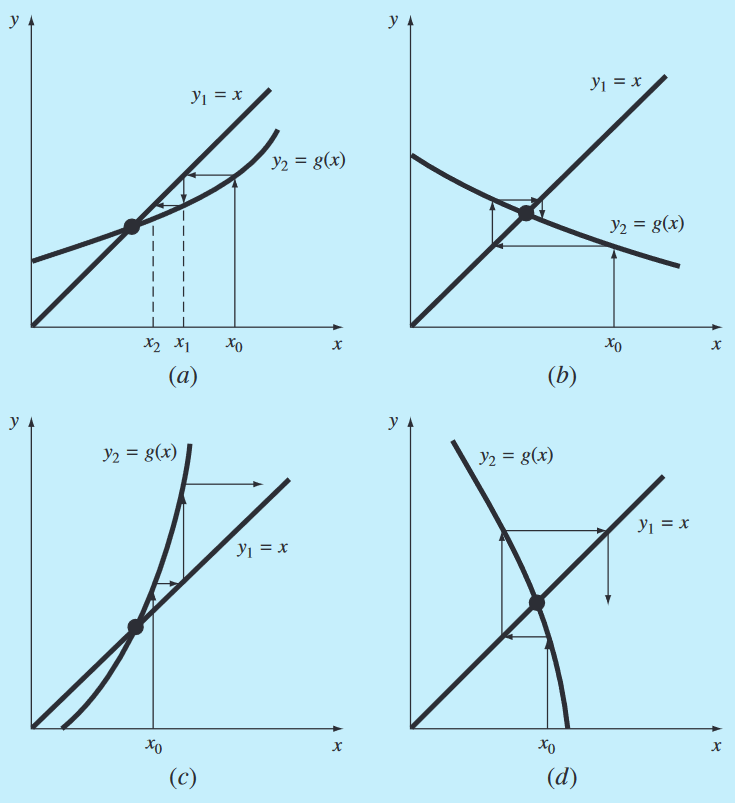
\includegraphics[width=0.5\textwidth]{fp_convergence.png}
    \end{center} 

\end{frame}

\begin{frame}{Dificultades con Punto Fijo}{Punto Fijo}
Si la pendiente de la función $g(x)$ es menor a la pendiente de la recta $y=x$ o sea, $|g'(x)| < 1$, entonces el método de punto fijo \alert{converge}.

\bigskip

Esta idea de que a partir de \textbf{la pendiente} podemos obtener más información, da pie a nuevos métodos y maneras de encontrar la raíz.
\end{frame}

\section{Newton-Raphson}

\begin{frame}{Repaso de cálculo}{Newton-Raphson}

    \begin{center}
        {\huge
        \textit{Throwback} a Cálculo Diferencial:}

        Secantes y Tangentes
    \end{center}

\end{frame}

\begin{frame}{El método de Newton-Raphson}{Newton-Raphson}
    El método de \alert{Newton Raphson} utiliza la recta \textbf{tangente} a uno de los puntos para determinar una aproximación de mejor calidad de una raíz. \pause

    \bigskip

    Como todos los procesos que hemos visto, utiliza la información de la aproximación actual (el día de hoy) para predecir la siguiente aproximación (del día de mañana) usando la derivada de la función, en una fórmula muy sencilla de recordar: \pause

    \begin{block}{Fórmula de Newton Raphson}
        $$x_{i+1} = x_i - \frac{f(x_i)}{f'(x_i)}$$
    \end{block}

\end{frame}

\begin{frame}{Ejemplo}{Newton-Raphson}
    Con la misma \textbf{función} anterior: $f(x) = e^{-x} - x$. \pause

    \bigskip

    ¿Cuál es la derivada de $f(x)$? \pause

    Usando la fórmula $\dv{e^u}{u} = e^u \cdot \dd{u}$, obtenemos que $f'(x) = -e^{-x} - 1$. \pause

    \bigskip

    Significa que para esta función, el próximo paso siempre se calculará como

    $$x_{i+1} = x_i - \frac{e^{-x_i} - x_i}{-e^{-x_i} - 1}$$

\end{frame}

\begin{frame}{Complicaciones}{Newton-Raphson}

    El método podría no converger\dots \pause

    \begin{itemize}
        \item \dots si la raíz está cerca de un punto de inflexión \pause
        \item \dots si se llega a algún punto con una pendiente de casi 0 \pause
        \item \dots si la pendiente de un punto es 0
    \end{itemize} \pause

    Por eso se sugiere tomar las acciones pertinentes para ello, como

    \begin{itemize}[<+->]
        \item Graficar la función
        \item Verificar que el resultado final esté realmente cerca de 0
        \item Incluir un \textbf{número máximo} de iteraciones
        \item Alertar cuando se encuentra una derivada muy cercana a 0
    \end{itemize}
\end{frame}

\begin{frame}{El método de la Secante}{Secante}

    El método de la \alert{secante} se basa en la misma idea que el método de \textbf{Newton-Raphson}, pero en lugar de considerar la recta tangente como aproximación, us a la recta secante. \pause

    \bigskip

    Para ello, utiliza \textbf{dos pasos} en el pasado (la info de hoy, y de ayer) para predecir el siguiente paso (el de mañana). \pause
    
    \bigskip

    La fórmula es muy parecida a la de \textbf{Newton-Raphson}, sin embargo la derivada se aproxima usando una diferencia:

    \begin{block}{Fórmula del método de la Secante}
        $$x_{i+1} = x_i - \frac{f(x_i)(x_{i-1} - x_i)}{f(x_{i-1}) - f(x_i)}$$
    \end{block}

\end{frame}

% What is control flow
% why is it important
% does it exist in math?
% how to represent it
% how to represent it in matlab
% practical cases

% \section*{Referencias}

% \begin{frame}[t]{Referencias}
    % \nocite{bibID01}
    % \nocite{bibID02}

    % \bibliographystyle{IEEE}
    % \bibliography{biblio}
% \end{frame}

\end{document}